\section{FSA-v4: The Variable-Dose Extension} \label{sec:fsa-v4}

Building upon the Bimodal Training Extension (FSA-v3), we now address a fundamental limitation of classical impulse-response models: the assumption of constant training sensitivity. As observed empirically, and formalized by Busso (2003), an athlete's response to a given training load is not static; it evolves based on their recent training history.

The FSA-v4 model captures this phenomenon by extending the state space to six dimensions. The previously static fatigue impulse coefficients ($\kappa_{FB}, \kappa_{FS}$) are promoted to dynamic latent states, denoted as $K_{FB}$ and $K_{FS}$.

\subsection{Dynamic Fatigue Sensitivity}

In the 6D SDE system $y(t) = (B, S, F, A, K_{FB}, K_{FS})^T$, the dynamic fatigue gains are governed by their own Stochastic Differential Equations:

\begin{align}
  \dd K_{FB} &= \left[ \frac{K_{FB}^0 - K_{FB}}{\tau_K} + \mu_K \Phi_B(t) \right] \dd t + \sigma_K \sqrt{K_{FB}} \dd W_{K_{FB}} \\
  \dd K_{FS} &= \left[ \frac{K_{FS}^0 - K_{FS}}{\tau_K} + \mu_K \Phi_S(t) \right] \dd t + \sigma_K \sqrt{K_{FS}} \dd W_{K_{FS}}
\end{align}

Here, $K_{Fi}^0$ represents the baseline fatigue sensitivity for modality $i$, $\tau_K$ is the recovery time constant for this sensitivity (typically $\approx 21$ days), and $\mu_K$ is the "damage" rate. 

\subsubsection{The Dual Effect of Training}
This formulation introduces a profound non-linearity into the control problem. Training stimuli $\Phi_B$ and $\Phi_S$ now possess a \textbf{dual effect}:
\begin{enumerate}
    \item \textbf{Direct Effect:} They immediately drive the accrual of fitness ($B$) and strength ($S$), while adding to the unified fatigue pool ($F$) proportionally to the current sensitivities $K_{FB}$ and $K_{FS}$.
    \item \textbf{Meta-Effect (Variable Dose):} They increase the sensitivity states $K_{FB}$ and $K_{FS}$ themselves (via the $\mu_K \Phi$ term). This means that training today makes the athlete \textit{more vulnerable} to fatigue from the same training load tomorrow.
\end{enumerate}

\subsection{Implications for the Concurrent Optimizer}

The introduction of dynamic fatigue sensitivity dramatically alters the Pareto front of concurrent training. 

In FSA-v3, the optimizer found a steady-state "Sustainability Zone" by balancing constant fatigue accumulation against the quadratic suppression of autonomic amplitude $A$. However, in FSA-v4, maintaining a constant high training load is no longer viable; the sensitivities $K_{FB}$ and $K_{FS}$ will rise, causing the fatigue pool $F$ to accelerate toward the collapse threshold $F_{\text{max}}$, even if the stimulus $\Phi$ remains unchanged.

To survive this, the model-predictive controller (MPC) must discover a higher-order form of periodization. It is forced to implement \textbf{deload weeks} or extended tapering phases. By temporarily dropping the stimulus $\Phi$ near zero, the controller allows the sensitivities $K_{FB}$ and $K_{FS}$ to decay back toward their baseline values ($K_{FB}^0, K_{FS}^0$), "resetting" the athlete's tolerance for the next heavy loading block.

Figure \ref{fig:horizon_study_v4} illustrates this advanced periodization strategy across extended horizons, demonstrating the controller's ability to manage the meta-effect of training sensitivity while still optimizing for the composite objective $J = -(A + B + S)$.

\begin{figure}[h]
    \centering
    \begin{tabular}{cc}
        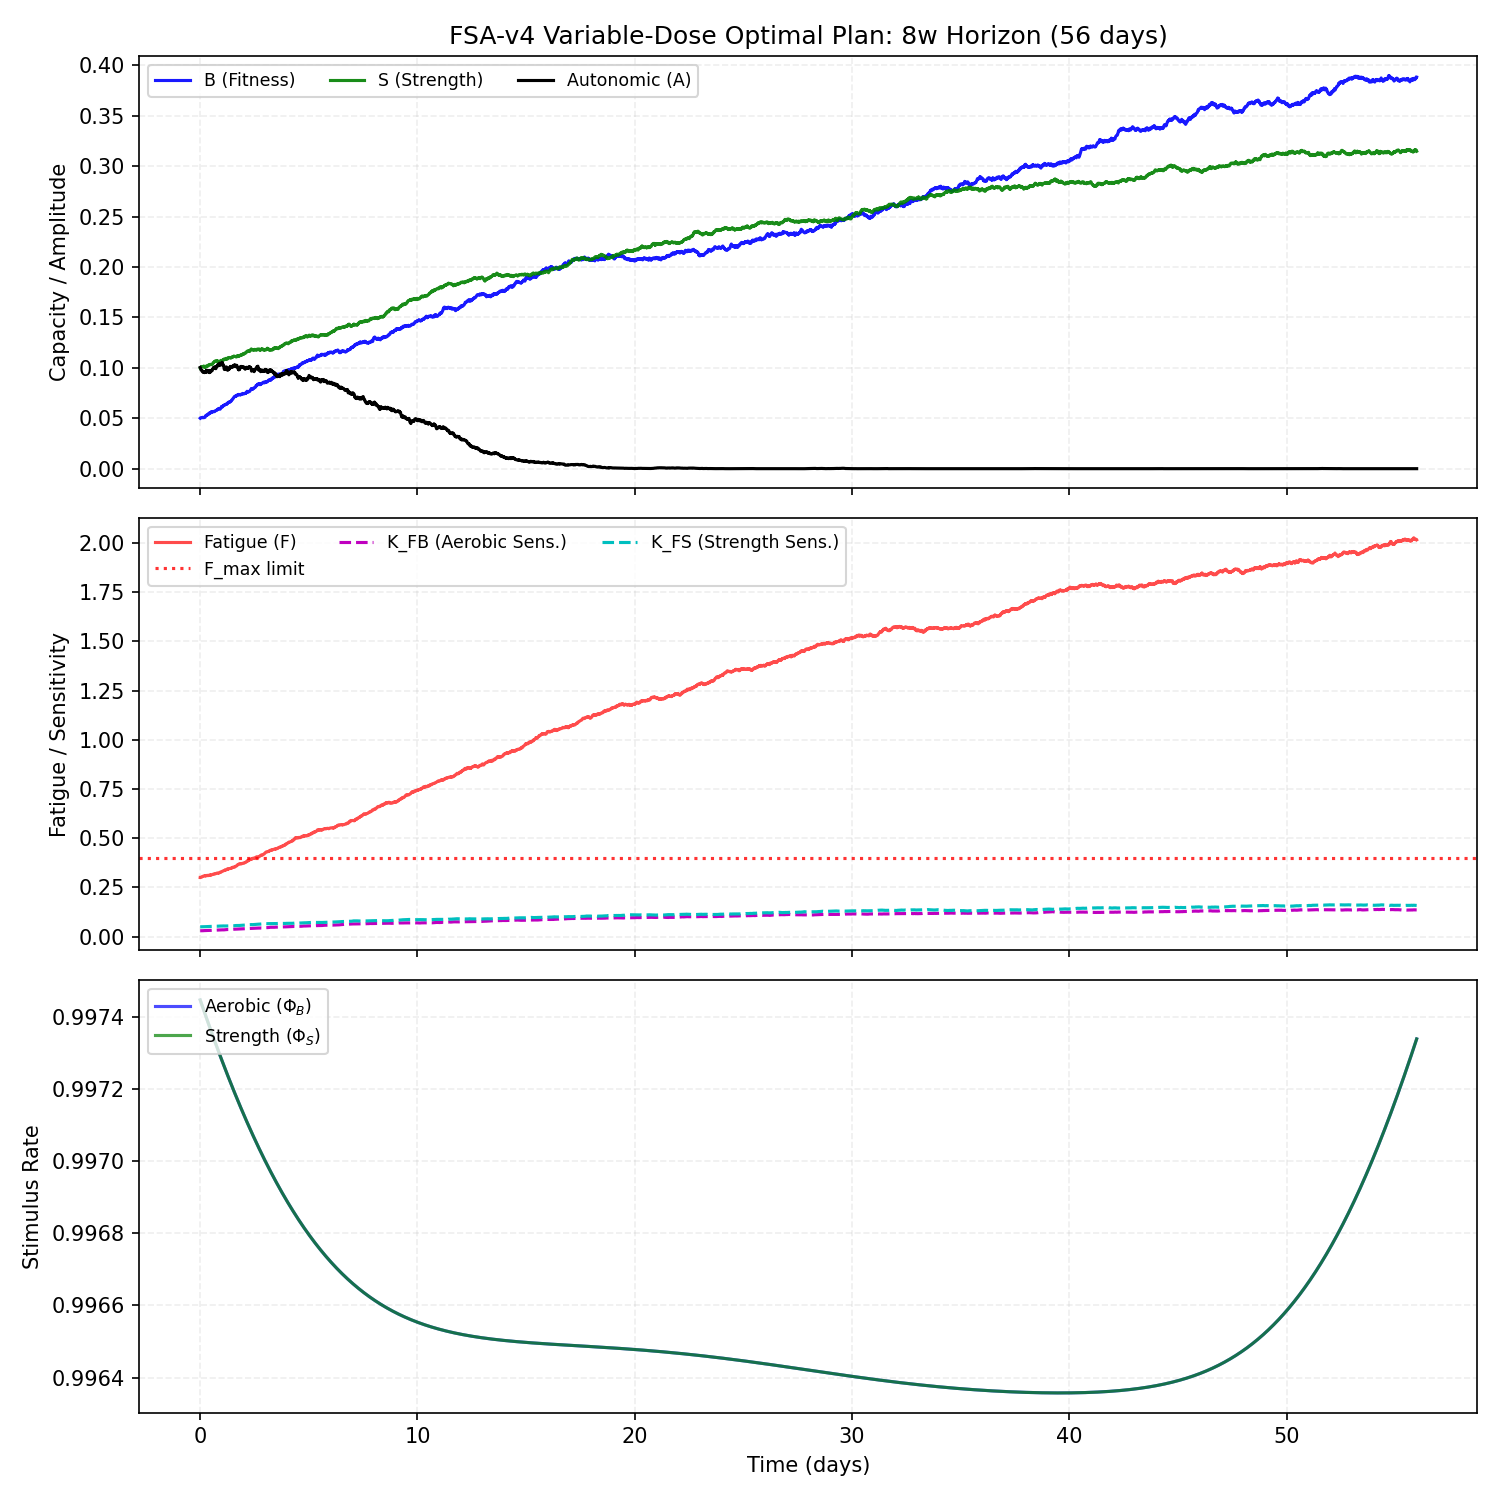
\includegraphics[width=0.48\textwidth]{figures/dynamic_transition_8w.png} & 
        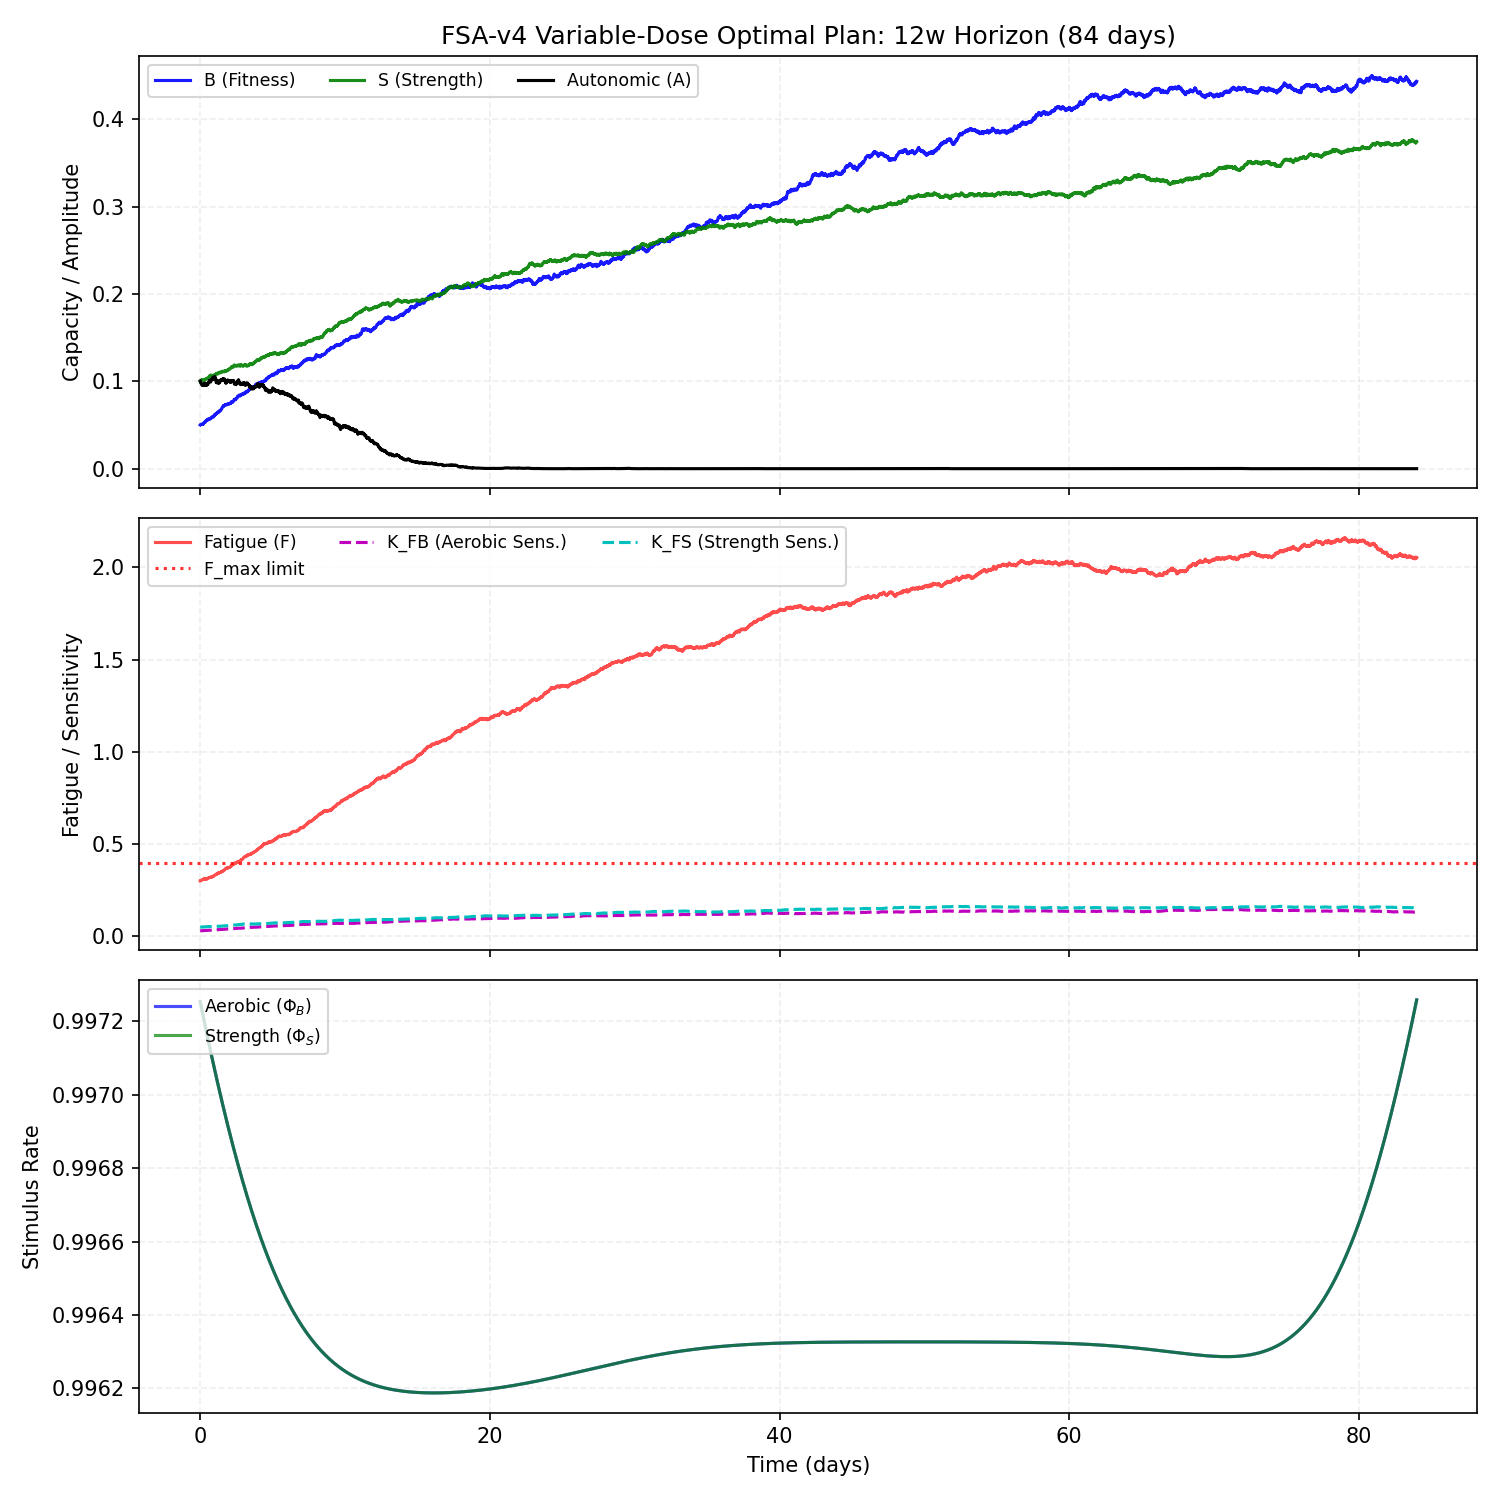
\includegraphics[width=0.48\textwidth]{figures/dynamic_transition_12w.png} \\
        (a) 8 Weeks (56 days) & (b) 12 Weeks (84 days) \\
        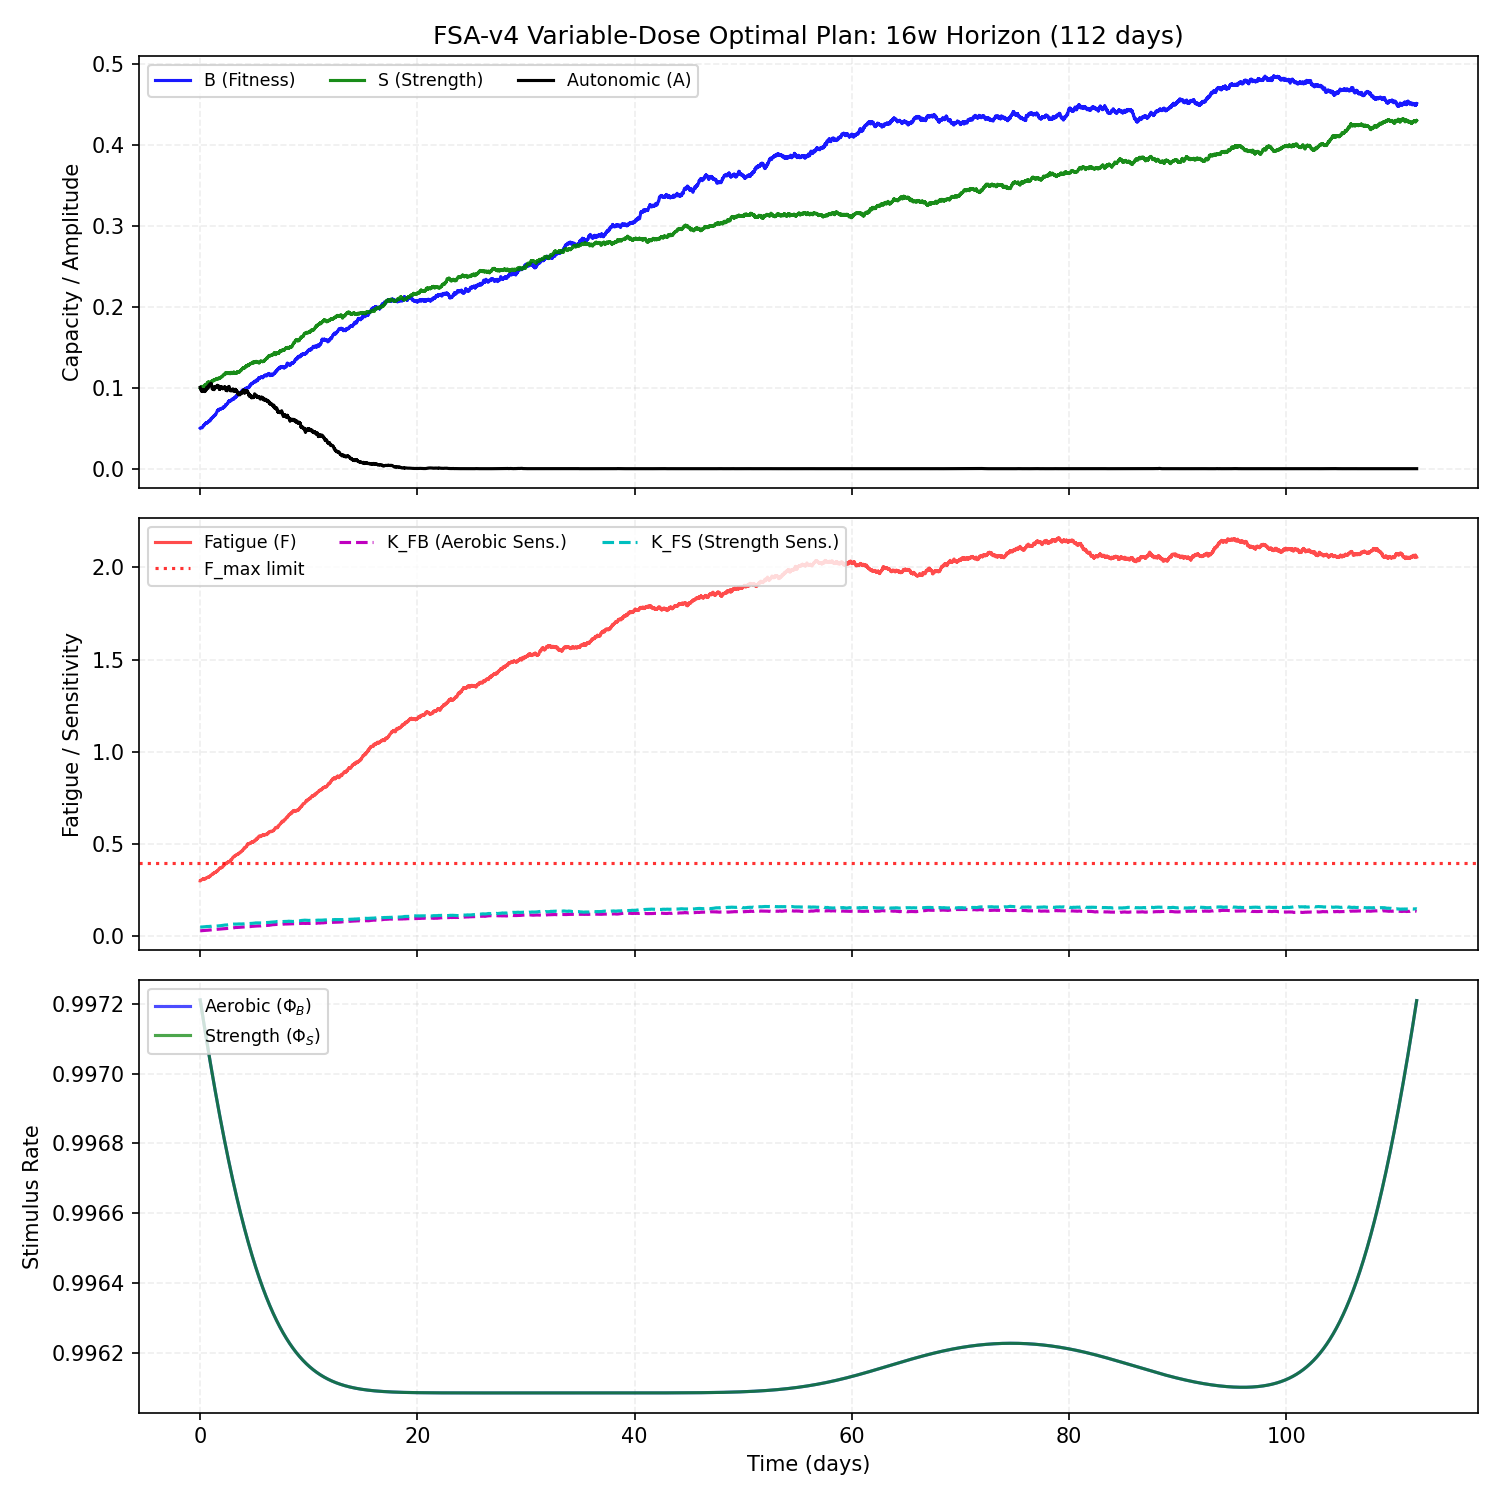
\includegraphics[width=0.48\textwidth]{figures/dynamic_transition_16w.png} & 
        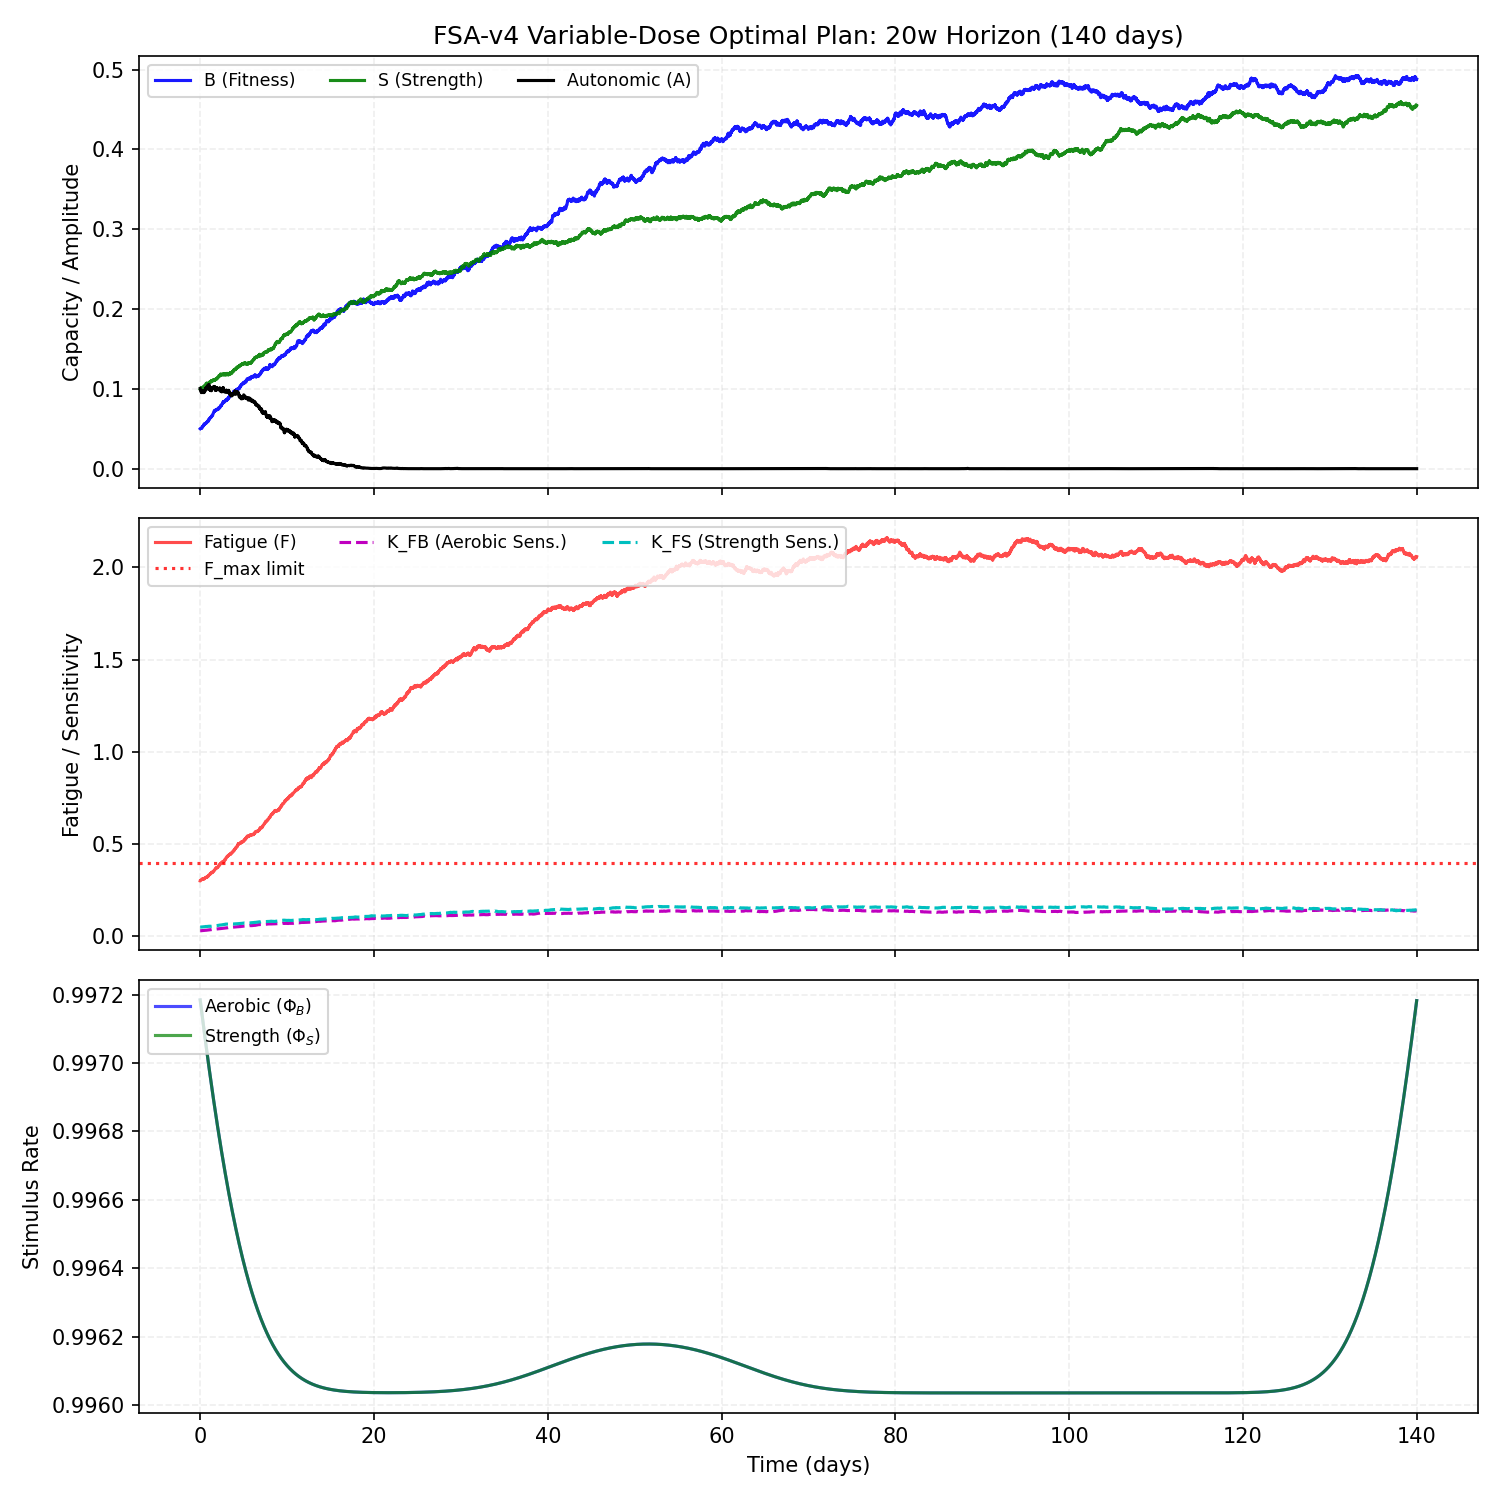
\includegraphics[width=0.48\textwidth]{figures/dynamic_transition_20w.png} \\
        (c) 16 Weeks (112 days) & (d) 20 Weeks (140 days)
    \end{tabular}
    \caption{FSA-v4 Variable-Dose Optimal Plans. The plots show the 6D latent state trajectory, including the dynamic fatigue sensitivities $K_{FB}$ and $K_{FS}$ (middle panels). Notice how prolonged loading causes $K_{FB}$ and $K_{FS}$ to rise, eventually forcing the controller to reduce stimulus to allow sensitivity recovery.}
    \label{fig:horizon_study_v4}
\end{figure}

\subsection{Parameter Estimation in the 6D SMC$^2$ Framework}

The promotion of $\kappa_{FB}$ and $\kappa_{FS}$ to dynamic states presents a novel challenge for the SMC$^2$ inference pipeline. In the static 4D model, the fatigue impulse gains could be identified from any reasonably varied training schedule. However, in the 6D Variable-Dose model, the parameters governing the sensitivity dynamics—specifically the damage rate $\mu_K$ and the recovery time constant $\tau_K$—are fundamentally unobservable if the training load remains constant.

\subsubsection{The Necessity of Excitement and Tapering}

To structurally identify the 6D model, the SMC$^2$ filter requires a highly informative observation record. The data must contain specific, contrasting phases:
\begin{enumerate}
    \item \textbf{Periods of High Excitement:} The athlete must undergo intense loading phases. Only when $\Phi$ is large does the $\mu_K \Phi$ term dominate, driving $K_{FB}$ and $K_{FS}$ significantly above their baselines. This provides the filter with the signal necessary to estimate the damage rate $\mu_K$.
    \item \textbf{Extended Taper or Deload Periods:} Following the excitement phase, the training load must drop significantly. During this deload, the sensitivities exponentially decay back to their baselines at a rate governed by $\tau_K$. Without this observable decay phase, the filter cannot separate the baseline sensitivity ($K_{Fi}^0$) from the time constant ($\tau_K$).
\end{enumerate}

Consequently, when utilizing the FSA-v4 model, rolling-window parameter estimation will be most accurate when analyzing macrocycles that include distinct, intentional periodization, validating the advanced schedules produced by our controller.
